% OA-RLAIF training-step detail (slides / README). Build: pdflatex -interaction=nonstopmode oa_rlaif_overview.tex
% PNG: pdftoppm -r 200 -png -singlefile oa_rlaif_training_step.pdf oa_rlaif_training_step ; SVG: pdftocairo -svg
\documentclass{article}
\usepackage[T1]{fontenc}
\usepackage{lmodern}
\usepackage{amsmath,amssymb}
\usepackage{tikz}
\usetikzlibrary{arrows.meta,positioning}
\renewcommand{\familydefault}{\sfdefault}
\definecolor{dFill}{HTML}{F1EFE8}\definecolor{dLine}{HTML}{5F5E5A}\definecolor{dText}{HTML}{2C2C2A}\definecolor{dSub}{HTML}{5F5E5A}
\definecolor{tFill}{HTML}{EEEDFE}\definecolor{tLine}{HTML}{534AB7}\definecolor{tText}{HTML}{26215C}\definecolor{tSub}{HTML}{3C3489}
\definecolor{gFill}{HTML}{E1F5EE}\definecolor{gLine}{HTML}{0F6E56}\definecolor{gText}{HTML}{04342C}\definecolor{gSub}{HTML}{085041}
\definecolor{oFill}{HTML}{FAECE7}\definecolor{oLine}{HTML}{993C1D}\definecolor{oText}{HTML}{4A1B0C}\definecolor{oSub}{HTML}{712B13}
\newcommand{\T}[2]{{\large\bfseries #1}\\[3pt]{\normalsize #2}}
\pagestyle{empty}
\setlength{\parindent}{0pt}\setlength{\textwidth}{50cm}\setlength{\textheight}{50cm}
\newsavebox\figbox
\begin{document}
\sbox\figbox{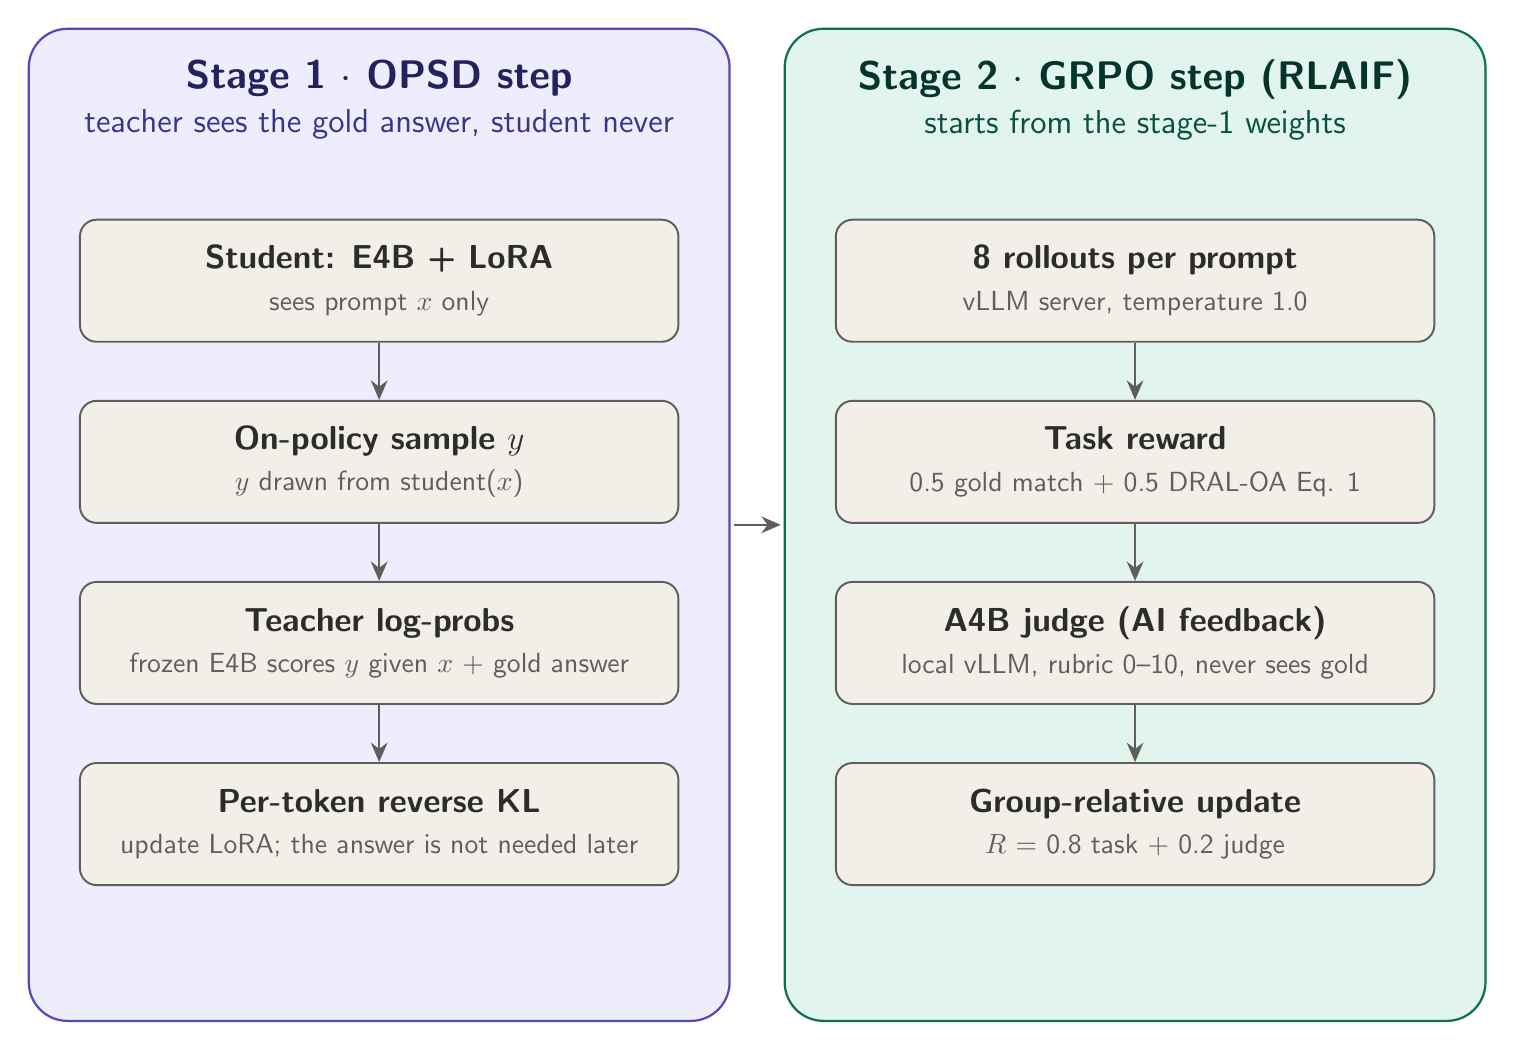
\begin{tikzpicture}[x=1cm,y=1cm, font=\sffamily, every node/.style={align=center},
  stepbox/.style={rounded corners=6pt, line width=0.7pt, fill=dFill, draw=dLine, text=dText, minimum width=7.6cm, minimum height=1.55cm},
  ar/.style={-{Stealth[length=7pt,width=6pt]}, line width=0.9pt, draw=dLine}]
\draw[rounded corners=14pt, line width=0.8pt, fill=tFill, draw=tLine] (0,0) rectangle (8.9,12.6);
\draw[rounded corners=14pt, line width=0.8pt, fill=gFill, draw=gLine] (9.6,0) rectangle (18.5,12.6);
\node[text=tText] at (4.45,11.7) {{\Large\bfseries Stage 1 $\cdot$ OPSD step}\\[4pt]{\large\color{tSub} teacher sees the gold answer, student never}};
\node[text=gText] at (14.05,11.7) {{\Large\bfseries Stage 2 $\cdot$ GRPO step (RLAIF)}\\[4pt]{\large\color{gSub} starts from the stage-1 weights}};
\node[stepbox] (a1) at (4.45,9.4) {\T{Student: E4B + LoRA}{\color{dSub}sees prompt $x$ only}};
\node[stepbox] (a2) at (4.45,7.1) {\T{On-policy sample $y$}{\color{dSub}$y$ drawn from student($x$)}};
\node[stepbox] (a3) at (4.45,4.8) {\T{Teacher log-probs}{\color{dSub}frozen E4B scores $y$ given $x$ + gold answer}};
\node[stepbox] (a4) at (4.45,2.5) {\T{Per-token reverse KL}{\color{dSub}update LoRA; the answer is not needed later}};
\node[stepbox] (b1) at (14.05,9.4) {\T{8 rollouts per prompt}{\color{dSub}vLLM server, temperature 1.0}};
\node[stepbox] (b2) at (14.05,7.1) {\T{Task reward}{\color{dSub}0.5 gold match + 0.5 DRAL-OA Eq. 1}};
\node[stepbox] (b3) at (14.05,4.8) {\T{A4B judge (AI feedback)}{\color{dSub}local vLLM, rubric 0--10, never sees gold}};
\node[stepbox] (b4) at (14.05,2.5) {\T{Group-relative update}{\color{dSub}$R$ = 0.8 task + 0.2 judge}};
\foreach \u/\v in {a1/a2,a2/a3,a3/a4,b1/b2,b2/b3,b3/b4} \draw[ar] (\u.south) -- (\v.north);
\draw[ar] (8.95,6.3) -- (9.55,6.3);
\end{tikzpicture}
}
\pdfpagewidth=\dimexpr\wd\figbox+24pt\relax
\pdfpageheight=\dimexpr\ht\figbox+\dp\figbox+24pt\relax
\hoffset=-1in \voffset=-1in
\shipout\vbox{\kern12pt\hbox{\kern12pt\usebox\figbox}}
\end{document}
